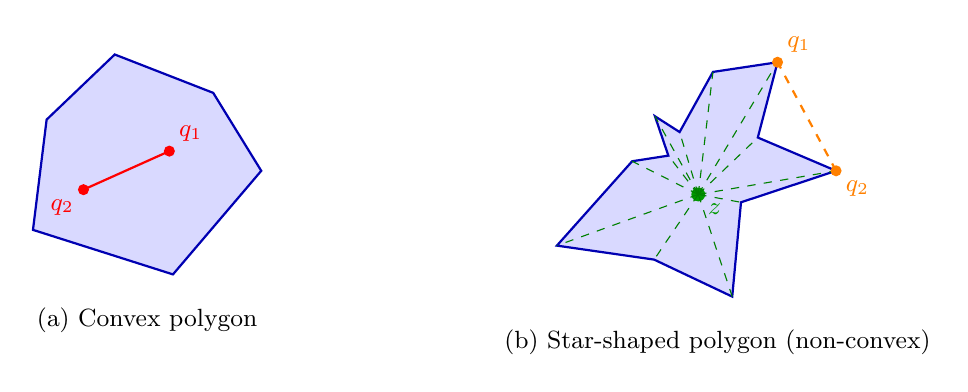
\begin{tikzpicture}
		% Left: Convex polygon
		\begin{scope}[shift={(-3.5,0)}, local bounding box=convex]
			\coordinate (A) at (0:1.6);
			\coordinate (B) at (45:1.4);
			\coordinate (C) at (100:1.5);
			\coordinate (D) at (150:1.3);
			\coordinate (E) at (210:1.5);
			\coordinate (F) at (290:1.4);

			\fill[blue!15] (A) -- (B) -- (C) -- (D) -- (E) -- (F) -- cycle;
			\draw[blue!70!black, thick] (A) -- (B) -- (C) -- (D) -- (E) -- (F) -- cycle;

			\fill[red] (30:0.5)  circle (2pt) node[above right, font=\small] {$q_1$};
			\fill[red] (200:0.7) circle (2pt) node[below left, font=\small]  {$q_2$};
			\draw[red, thick] (30:0.5) -- (200:0.7);

			\node[below, yshift=-0.3cm] at (convex.south) {\small (a) Convex polygon};
		\end{scope}

		% Right: Star-shaped polygon (non-convex, jagged)
		\begin{scope}[shift={(3.5,0)}, local bounding box=starshaped]
			% Jagged star-shaped polygon (irregular, concave indentations on right side)
			\coordinate (S0)  at (  0:1.9);
			\coordinate (S1)  at ( 25:1.0);
			\coordinate (S2)  at ( 50:1.8);
			\coordinate (S3)  at ( 75:1.3);
			\coordinate (S4)  at (100:0.5);
			\coordinate (S5)  at (120:0.8);
			\coordinate (S6)  at (140:0.3);
			\coordinate (S7)  at (170:0.7);
			\coordinate (S8)  at (210:1.9);
			\coordinate (S9)  at (250:1.2);
			\coordinate (S10) at (290:1.7);
			\coordinate (S11) at (330:0.8);

			\fill[blue!15] (S0) -- (S1) -- (S2) -- (S3) -- (S4) -- (S5) -- (S6) -- (S7) -- (S8) -- (S9) -- (S10) -- (S11) -- cycle;
			\draw[blue!70!black, thick] (S0) -- (S1) -- (S2) -- (S3) -- (S4) -- (S5) -- (S6) -- (S7) -- (S8) -- (S9) -- (S10) -- (S11) -- cycle;

			% Kernel point z
			\coordinate (Z) at (0.15, -0.3);
			\fill[green!60!black] (Z) circle (2.5pt) node[below right, font=\small] {$z$};

			% Rays from kernel z to all boundary vertices
			\foreach \i in {0,...,11} {
				\draw[green!50!black, dashed, thin] (Z) -- (S\i);
			}

			% Two interior points whose segment exits the polygon (non-convexity)
			\fill[orange] (S2)  circle (2pt) node[above right, font=\small] {$q_1$};
			\fill[orange] (S0) circle (2pt) node[below right, font=\small] {$q_2$};
			\draw[orange, thick, dashed] (S0) -- (S2);

			\node[below, yshift=-0.3cm] at (starshaped.south) {\small (b) Star-shaped polygon (non-convex)};
		\end{scope}
	\end{tikzpicture}
